\documentclass[11pt]{article}

\usepackage[T1]{fontenc}
\usepackage[utf8]{inputenc}
\usepackage[spanish]{babel}
\usepackage[letterpaper,
            portrait,
            margin=2cm]{geometry}
\usepackage{graphicx}
\usepackage{textcomp}
\usepackage{enumerate}
\usepackage{enumitem}
\usepackage{alltt}
\usepackage{import}

\setlist[itemize]{noitemsep, topsep=0pt}

\newcommand{\bt}{\begin{alltt}}
\newcommand{\et}{\end{alltt}}
\newcommand{\comando}[2]{
    \textbf{#1}(#2)\\
}

\newenvironment{args}{
    \newline
    Argumentos:
    \begin{itemize}
}{
    \end{itemize}
    \bigskip
}

\setlength{\parindent}{0pt}

\title{Inteligencia Artificial 2018-1 \\ Proyecto 2: Búsqueda\\
\vspace{2mm}
\small{IIMAS-PCIC}}
\author{Luis Alejandro Lara Patiño\\Roberto Monroy Argumedo\\
Alejandro Ehécatl Morales Huitrón}
\date{23 de noviembre de 2017}


\begin{document}

\maketitle

\tableofcontents

\section{Funcionamiento del proyecto}

\subsection{Carga de información}
Toda la información necesaria para el funcionamiento del programa debe cargarse en la base de conocimiento previamente a la ejecución. Las bases se guardan en el directorio \texttt{bases}, y se pasan como argumento al programa escribiendo el nombre de archivo, sin la extensión.

\subsection{Ejecución}

El punto de entrada al proyecto es el archivo main.pl. Este archivo está acondicionado para ejecutarse tanto desde el listener de Prolog como desde una terminal en sistemas operativos UNIX.

\subsubsection{Desde una terminal UNIX}
El archivo main.pl puede ejecutarse como cualquier otro \textit{script}; solamente se debe navegar hasta el directorio del proyecto y desde allí ejecutar el comando:

\bt
    ./main.pl <nombre-base>
\et

\subsubsection{Desde el listener de Prolog}
Asimismo, es posible ejecutar el programa desde el entrono de Prolog. Para ello, se debe consultar el archivo main.pl, y realizar la siguiente consulta:

\bt
    ?- main([<nombre-base>])
\et

\section{Estructura de la base de conocimiento}

La estructura de base de conocimiento que utiliza este proyecto puede dividirse en tres secciones principales: conocimiento conceptual, conocimiento factual y conocimiento del mundo.

\subsection{Conocimiento conceptual}

En esta sección se almacena la información acerca de los objetos que participan en las actividades del robot. En el caso del asistente de supermercado, aquí se almacenan los productos de la tienda en forma de objetos, los cuales heredan las propiedades y relaciones de sus clases padre de acuerdo a la jerarquía implementada en el primer proyecto.

\subsection{Conocimiento factual}

En esta sección se almacenan las acciones realizables tanto por el empleado de la tienda como por el robot. También se mantienen aquí las decisiones que puede tomar el robot, así como la creencia que tiene el robot del mundo y las observaciones que éste adquiere durante la ejecución del programa.

Finalmente, se almacenan aquí los resultados de cada uno de los módulos del proyecto, dentro de los objetos \texttt{diagnostico}, \texttt{decision} y \texttt{agenda}.

\subsection{Conocimiento del mundo}

En esta sección se guarda la configuración que tiene el mundo del robot; las ubicaciones a las que éste puede acceder y qué objetos hay actualmente en ellas.

También existe un objeto \texttt{robot}, que mantiene los objetos que éste tiene en sus brazos y la posición en la que se encuentra.

\section{Módulos}

\subsection{Simulador}

La primera sección del proyecto que se ejecuta cuando éste inicia es el simulador. Éste se encarga de coordinar la ejecución de los tres módulos cuando sea necesario y de ejecutar el plan encontrado.

Al inicio del programa, el simulador ejecuta los tres módulos para generar un plan y cumplir las órdenes del cliente. En esta primera iteración, el robot confía plenamente en el reporte inicial del empleado de la tienda, y solamente busca entregar los productos que el cliente le pidió.

Una vez generado el plan, el simulador ejecuta las acciones secuencialmente. para determinar si una acción tuvo o no éxito, se extrae la probabilidad de éxito de la misma, almacenada en la base de conocimiento y mediante un generador de números aleatorios, se aplica dicha probabilidad. Adicionalmente, la acción buscar puede fallar si se recibe una observación que no concuerda con la creencia que tiene el robot del mundo en ese momento.

Si alguna de las acciones falla, el simulador vuelve a ejecutar los tres módulos del proyecto, con el fin de generar un nuevo plan para superar los obstáculos que pueda haber encontrado. Las acciones anteriores se repiten hasta que el robot cumple con todas sus encomiendas. En este momento, el programa termina.

\subsection{Módulo de diagnóstico}

Para hacer un dignostico se necesita un conjunto de observaciones y una
locación actual. También una lista de objetos y posiciones restantes.
La forma en como se obtiene es realizando una búsqueda en la que en cada
paso agregamos una acción ´´mover'' o ´´colocar'' hasta que la lista de
objetos y posiciones restantes sea vacíá en cuyo caso agregamos la
locación inicial para así obtener (en una lista) el conjunto de acciones
de final a principio que realizó el almacenista.

La forma de nuestra función sucesor toma en cuenta la minima falla que pudo
cometer el almacenista, es decir suponemos que los productos están en su
lugar.

\subsection{Módulo de toma de decisión}

\subsection{Módulo de planeación}

La entrada al módulo de planeación son las decisiones que se tomaron en el módulo anterior. Éstas son los objetivos que debe cumplir el plan generado por este módulo.

Para representar un camino en el árbol de búsqueda, se utilizó una estructura de datos llamada nodo, la cual tiene tres campos: el primero indica el estado inicial de dicho camino. El segundo campo consiste en una lista de acciones que forman el camino. Finalmente, el tercer campo contiene el estado final alcanzado tras seguir la secuencia de acciones desde el estado inicial.

Para codificar un estado, se empleó una lista. Dicha lista contiene la configuración del robot en ese instante, y listas para cada ubicación en el mundo, que indican los objetos presentes en cada una de ellas.

El algoritmo utilizado en este módulo es una versión modificada del algoritmo de búsqueda primero el mejor. Éste explora una gráfica utilizando dos conjuntos de nodos: los "blancos", o ya explorados, y los "grises", también llamados "frontera", que son aquellos nodos expandidos, pero que aún no han sido explorados. En cada iteración, este algoritmo toma el mejor nodo de los grises; en este caso, el que ofrece la mayor recompensa, y lo expande. Los sucesores expandidos se guardan en el conjunto de los grises, y el nodo extraído se guarda en los blancos. Si el nodo seleccionado cumple alguno de los objetivos, dicho objetivo se elimina de la lista actual y se continúa la búsqueda para cumplir los restantes. El algoritmo termina cuando ya no queda ningún objetivo por cumplir.

El algoritmo implementado en este proyecto tiene algunas particularidades que es importante mencionar:

En cada iteración del algoritmo, las acciones expandidas no corresponden a todas las acciones realizables por el robot, sino solamente aquellas aplicables al estado actual. Por ejemplo, la acción agarrar no será expandida si en la acción anterior no se buscó un objeto. La acción colocar será expandida solamente para objetos que el robot tenga en sus manos. De esta manera, se limita el árbol de búsqueda sólo a acciones completamente posibles, disminuyendo el tiempo necesario para encontrar un plan y la memoria utilizada.

El principal criterio para elegir un nodo es la recompensa que éste obtiene. El cálculo de la recompensa se basa en la última acción en el camino desde la raíz hasta el nodo en cuestión. Si la misma acción ya se realizó con los mismos argumentos, significa que posiblemente el plan esté atascado en un ciclo de acciones. Por lo tanto, no se recompensa este tipo de acciones. Además, si una misma acción contribuye a cumplir más de un objetivo, se incrementa la recompensa que se le asigna, dando mayor prioridad a los objetivos más inmediatos.

\subsubsection{Ejemplo de ejecución}

Para mostrar el funcionamiento de este módulo, se analizará el caso en el cual el módulo de decisión obtuvo el objetivo de entregar el objeto \texttt{refresco1} al cliente. Este objeto, como reportó el empleado, se encuentra en la ubicación llamada \texttt{e1}. El robot se encuentra actualmente en la posición \texttt{inicio}, y no trae nada en sus manos.

El árbol de búsqueda generado en este caso se muestra en la figura~\ref{fig:ArbolPlaneacion}. En esta figura se muestra cada estado como un rectángulo que contiene cuatro círculos; uno por cada ubicación posible para el robot. Se marca con un círculo negro el objeto de interés, en este caso \texttt{refresco1}. La posición del robot se marca con un triángulo.

\begin{figure}
    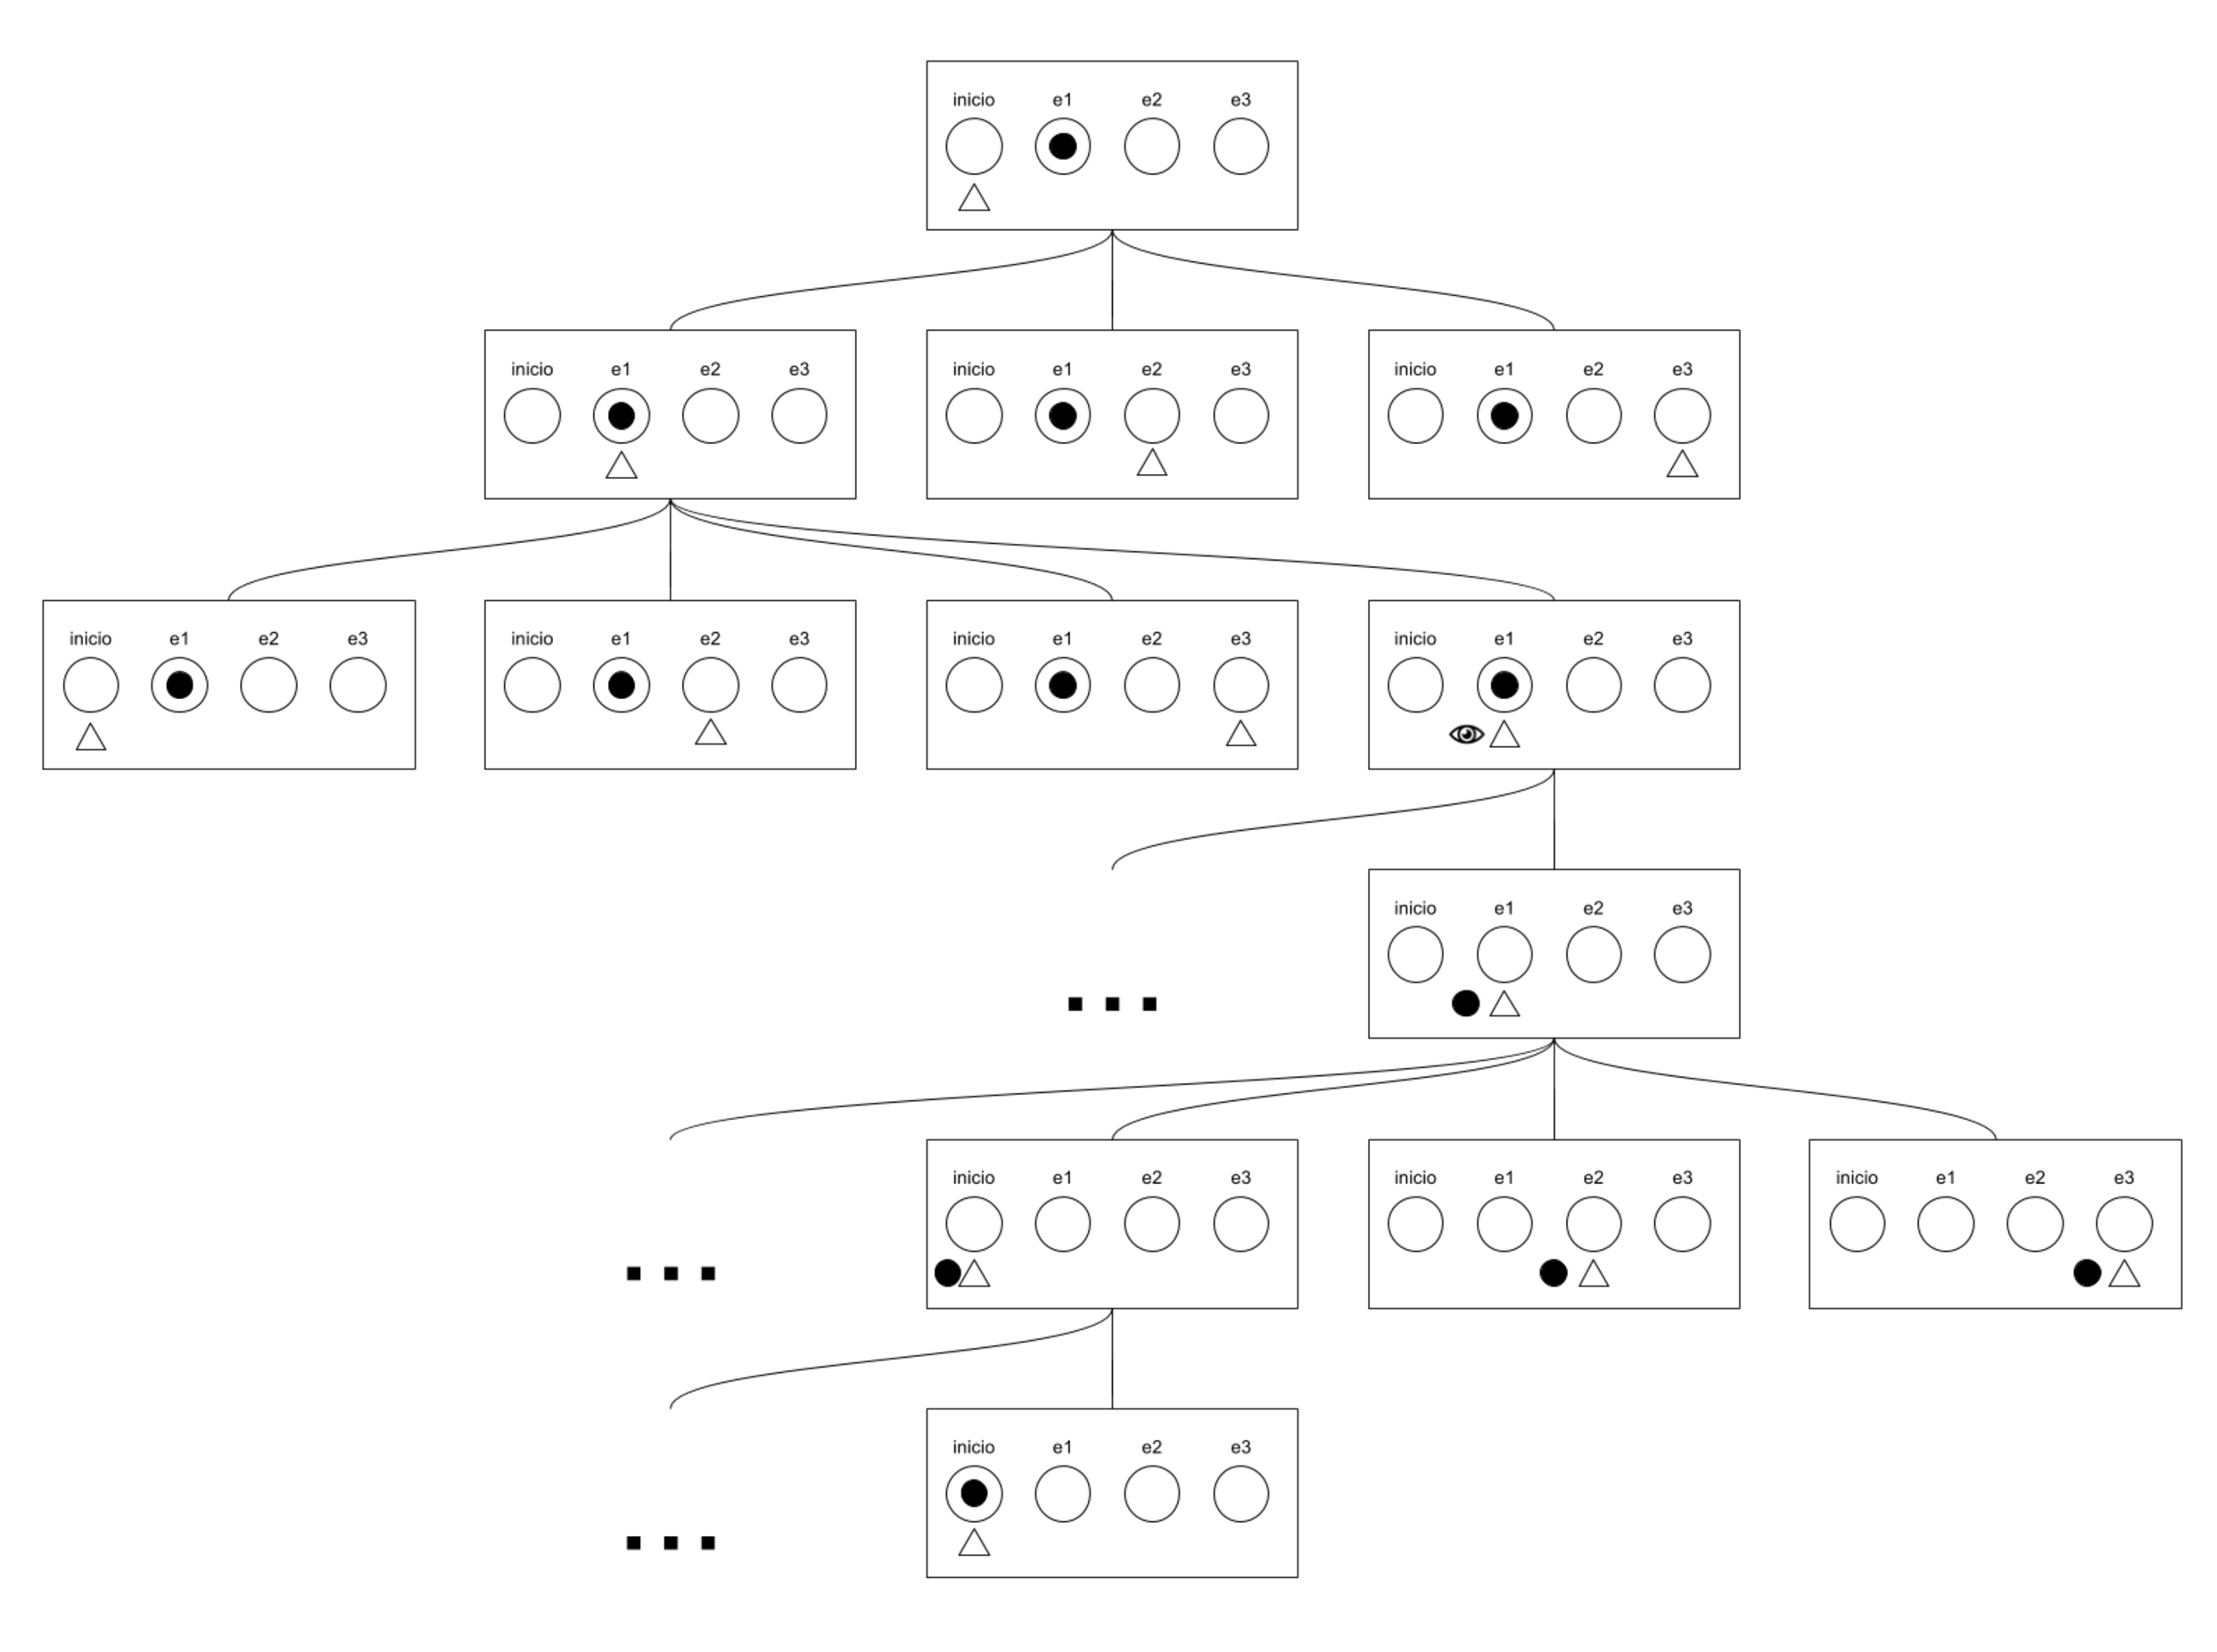
\includegraphics [width = \textwidth] {img/ArbolPlaneacion}
    \caption{Árbol de búsqueda del módulo de planeación.}
    \label{fig:ArbolPlaneacion}
\end{figure}

La raíz del árbol de búsqueda es el estado inicial, tal como se describió arriba. De acuerdo a las reglas establecidas en esta sección, desde este estado solamente es posible realizar la acción mover. No puede realizarse la acción agarrar, porque no se ha buscado ningún objeto; tampoco la acción buscar porque no hay objetos en la ubicación actual. La acción colocar es imposible porque el robot no tiene nada en sus brazos. Como hijos del estado inicial se muestran los tres estados resultantes de llevar a cabo la acción mover a cada una de las ubicaciones restantes.

En la siguiente iteración, el algoritmo debe elegir uno de los sucesores para ser expandido. Los dos últimos hijos no contribuyen a alcanzar el objetivo, por lo que no reciben recompensa. El único hijo que recibe recompensa es el primero, por lo que es el que se elige. Se observa que a partir de este estado es posible expandir nuevamente la acción mover. También es posible realizar la acción buscar, ya que hay objetos en la ubicación actual, según la creencia del robot. Se generará un sucesor por cada objeto que haya en la ubicación actual, pero solamente se muestra aquí una instancia, marcada con ícono de ojo.

En esta ocasión, dos acciones reciben recompensa: buscar y mover a inicio. Es incluso posible que mover a inicio reciba una mayor recompensa que buscar. Sin embargo, al elegir la primera, ninguno de sus sucesores recibe recompensa, por lo que se quedarán en la frontera hasta que todos los nodos grises tengan recompensa 0. Por lo tanto, la acción buscar será seleccionada antes que cualquier sucesor de mover a inicio.

Ya que en cualquier momento es posible expandir la acción mover, se omitieron dichos nodos por brevedad. En este caso es posible aplicar la acción agarrar, ya que el objeto se buscó en la acción inmediata anterior. Se observa que, en todos los sucesores de la acción agarrar, el robot ya tiene el objeto deseado en su posesión. Se muestran los sucesores que consisten en la acción mover, pero también es posible buscar otro objeto. Como esta última acción no contribuye a alcanzar el objetivo actual, no recibe recompensa.

En la siguiente iteración, la acción mover a inicio es la única que recibe recompensa. Podría objetarse que ésta ya se expandió anteriormente, y que no debería recibir recompensa, pero aquello ocurrió en otro camino desde la raíz. En este camino en particular, es la primera ocasión en la que se expande la acción mover a inicio, por lo que sí recibe recompensa.

Una vez en la posición inicio, la única acción recompensada del robot es colocar el refresco en la posición de inicio, que en este caso significa la entrega al cliente.

Como este estado cumple el objetivo planteado y no existen más objetivos por cumplir, la búsqueda se detiene y se regresa el plan encontrado.

\subsection{Utilitarios}

\end{document}
